\section{Differenz-Ableitung}
\label{sec:diff:derivation}

Die Differenz-Ableitung ist der zweite Schritt zur Berechnung einer symmetrischen Differenz zwischen
Modell A und B. In diesem Schritt werden die Objekte identifiziert, die nicht in der Schnittmenge
der beiden Modell sind. Die so berechnete Differenz wird im Folgenden als \textbf{technische
Differenz} bezeichnet. Eine technische Differenz teilt sich zunächst in zwei Klassen ein:
\texttt{Correspondence} und \texttt{Change}. Die zuvor im Matching berechneten Korrespondenzen der
Schnittmenge werden durch Objekte der Klasse \texttt{Correspondence} dargestellt. Die Summe aller
\texttt{Correspondence} gibt damit die gemeinsamen Teile von Modell A und Modell B an. Die Teile,
die sich von Modell A zu Modell B unterscheiden, werden durch Objekte der Klasse \texttt{Change}
(Änderung) angegeben. Bei Änderungen an einem Modell unterscheiden wir dabei noch zusätzlich
zwischen den drei Grundelementen eines Modells: Objekte, Referenzen und Attribute. Objekte und
Referenzen können in ein Modell sowohl eingefügt als auch entfernt werden. Ausgehen davon, dass wir
keine mehrwertigen Attribute betrachten, sind hingegen einwertige Attribute durch die Metaklassen
fest vorgegeben und können daher nur einen neuen Wert zugewiesen bekommen. Zu diesem Zweck werden
folgende Klassen definiert:

\begin{itemize}
  \item \texttt{Add-Object}: In Modell B existiert ein Objekt, welches nicht in Modell A existiert.
  Das Objekt wurde also in Modell B hinzugefügt.
  
  \item \texttt{Remove-Object}: In Modell A existiert ein Objekt, welches nicht in Modell B
  existiert. Das Objekt wurde also in Modell B entfernt.
  
  \item \texttt{Add-Reference}: In Modell B existiert eine Referenz, welche nicht in Modell A
  existiert. Die Referenz wurde also in Modell B hinzugefügt.
  
  \item \texttt{Remove-Refernce}: In Modell A existiert eine Referenz, welche nicht in Modell B
  existiert. Die Referenz wurde also in Modell B entfernt.
  
  \item \texttt{Attribute-Value-Change}: Für alle Objekte aus Modell A und Modell B, für die eine
  Korrespondenz existiert, wird überprüft, ob sich der Wert eines Attributs verändert hat und ggf.
  ein Attribute-Value-Change erzeugt. Es werden keine Attribute-Value-Changes für neue
  initialisierte Attribute eines Add-Objects angelegt.
  
  Attribute, deren Metatyp (\texttt{EAttribute}) folgende Eigenschaften haben, können dabei
  vernachlässigt werden, da sich aus diesen Attributen keine direkten Änderungen des Modells
  ableiten lassen:
  
  \begin{itemize}
    \item\texttt{changeable = false} $\to$ Der Wert kann von außen nicht verändert werden. D.h. es
    wird keine \texttt{setXX()} Methode generiert. \cite{SBPM2009} (S. 108)
    
    \item\texttt{transient = true} $\to$  Der Wert wird bei der Serialisierung übergangen und nicht
    mit abgespeichert. \cite{SBPM2009} (S. 108)
    
    \item \texttt{derived = true} $\to$ Gibt an, dass dieser Wert aus anderen Informationen
    abgeleitet wird. Hat aber keinen Einfluss auf die Code Generierung. \cite{SBPM2009} (S. 108)
  \end{itemize}
\end{itemize}
Das in Ecore Implementierte Differenzmodell ist in Abbildung \ref{fig:diffmodel} zu sehen. Es bildet
die Basis für das spätere Semantic-Lifting. Die in dieser Phase berechneten \texttt{Changes} werden
im Folgenden als \textbf{low-level Änderungen} bezeichnet, da die durchgeführten Änderungen am
Modell hier noch auf einer rein technischen Ebene angegeben werden.

\begin{figure}[htb]
  \centering
  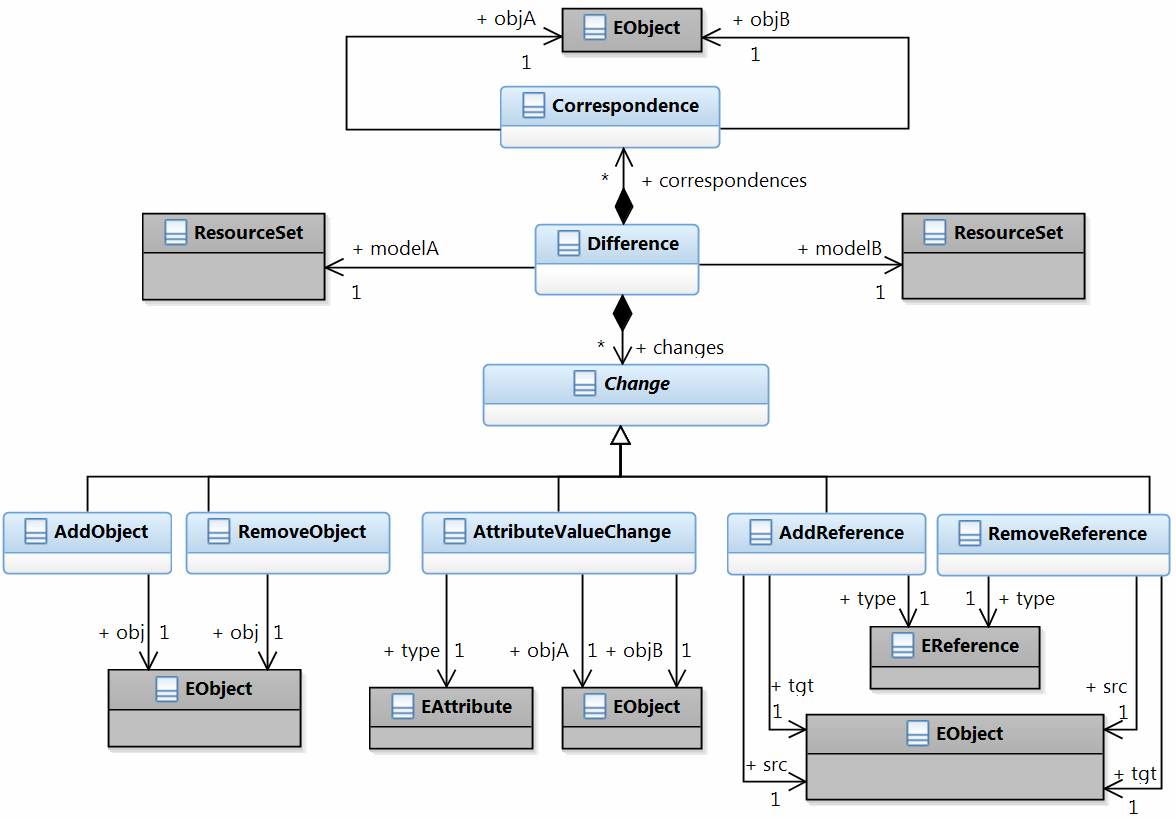
\includegraphics[width=1.0\textwidth]{images/difference_model.png}
  \caption{Differenzmodell}
  \label{fig:diffmodel}
\end{figure}